\section{Experiments}\label{sec:experiment}
In this section, we study our solutions for sketch discovery in both offline and online scenarios using the following four real datasets with statistics being summarized in Table~\ref{tbl:dataset}.

\noindent\textbf{NBA}\footnote{http://www.nba.com} contains the game records for each NBA player from year $1985$ to $2013$. Among all the records, we pick $1,000$ players with at least $200$ game records. In total, we obtain a dataset with $569$K events.

\noindent\textbf{POWER}~\cite{Lichman2013} contains the electricity usage for 370 households between Dec. 2006 and Nov. 2010. Each household is treated as a subject with the daily power usage as an event. In total, there are 1.4M events.

\noindent\textbf{PEMS}~\cite{choe2002freeway} contains the occupancy rate of freeway in San Francisco bay area from Jan. 2008 to Mar. 2009. Each freeway is a subject with the daily occupancy rate as an event. The dataset contains 963 freeways with 5.7M events.

\noindent\textbf{STOCK} contains the hourly price tick for 318 stocks from Mar. 2013 to Feb. 2015.
The dataset is crawled from Yahoo! Finance\footnote{https://finance.yahoo.com/} and contains 2.3M events.

 
{\renewcommand{\arraystretch}{1.2} 
\begin{table}[h]
\caption{Statistics of datasets used in experiments}
\centering
\begin{tabular}{|c|c|c|c|}
\hline
DataSet & Total Events & Total Subjects  & Longest Window \\
\hline
NBA & 569,253 & 1,015&  1,476 \\
\hline
POWER & 1,480,000 & 370 & 4,000 \\
\hline
PEMS & 5,798,918 & 963&  6,149 \\
\hline
STOCK & 2,326,632 & 318&  10,420 \\
\hline
\end{tabular}
\label{tbl:dataset}
\end{table}
}

%\begin{table}[h]
%\caption{Parameter Settings in Experiments }
%\centering
%\begin{tabular}{c|l}
%\hline
%$p$ & 20, 40, 80, 120, 160, \textbf{200} \\ 
%\hline
%$h$ & 20, 40, 60, 80, \textbf{100} \\
%\hline
%$k$ & \textbf{20}, 40, 60, 80, 100  \\
%\hline
%\end{tabular}
%\label{tbl:parameters}
%\end{table}

In our efficiency study, we evaluate three parameters: 1) $p\in[20,200]$, which refers to the worst rank for an event window to become a candidate theme, 2) $k\in[20,100]$, which refers to the number of candidate themes in a sketch and 3) $h\in[20,100]$, which refers to the percentage of historical events for scalability test, i.e. $|\mathbb{H}|\cdot h\%$ events are used in the experiments. We use $p=200$, $h=100$ and $k=20$ as the default values.

All the experiments are conducted on a desktop machine equipped with an Intel i7 Dual-Core 3.0GHz CPU, 8GB memory and 160 GB hard drive. All algorithms are developed using Java 7. 
 
\subsection{Offline Sketch Discovery}
\label{subsec:exp-offline}
Our offline sketch discovery algorithms consist of two functional components, \emph{Candidate Theme Generation}
and \emph{Sketch Discovery}. In the candidate theme generation, we report the performance with varying $p$ and $h$. In the sketch discovery, we report the performance with varying $k$.

\subsubsection{Candidate theme generation algorithms}
To evaluate the performance, we design the following four methods for comparison:

\noindent\textbf{Brute-Force (BF)}: BF exhaustively computes and compares for each subject all the possible window lengths. 

\noindent\textbf{Visiting-Window Pruning (V-WP)}: V-WP only adopts the \emph{visiting-window} bound for pruning.

\noindent\textbf{Unseen-Window Pruning (U-WP)}: U-WP only adopts the \emph{unseen-window} bound for pruning. 

\noindent\textbf{Unseen+Visting Window Pruning (UV-WP)}: UV-WP adopts both \emph{unseen-window} pruning and \emph{visiting-window} pruning.

\subsubsection{Candidate themes generation with varying $p$}
The running time of the four algorithms in candidate theme generation wrt. $p$ is shown in Fig.~\ref{exp:offline_performance_vary_p}. It is evident that when $p$ increases, more candidate themes are qualified and thus all four algorithms require more computation time. The effect of the two proposed window-based pruning techniques can also be observed from the figure. The insight is that the unseen-window pruning plays a more important role in reducing the running time. Furthermore, when both pruning techniques are used, our method achieves at least two orders of magnitude of performance improvement.

\begin{figure*}[t]
\centering
    \begin{subfigure}[b]{0.45\textwidth}
        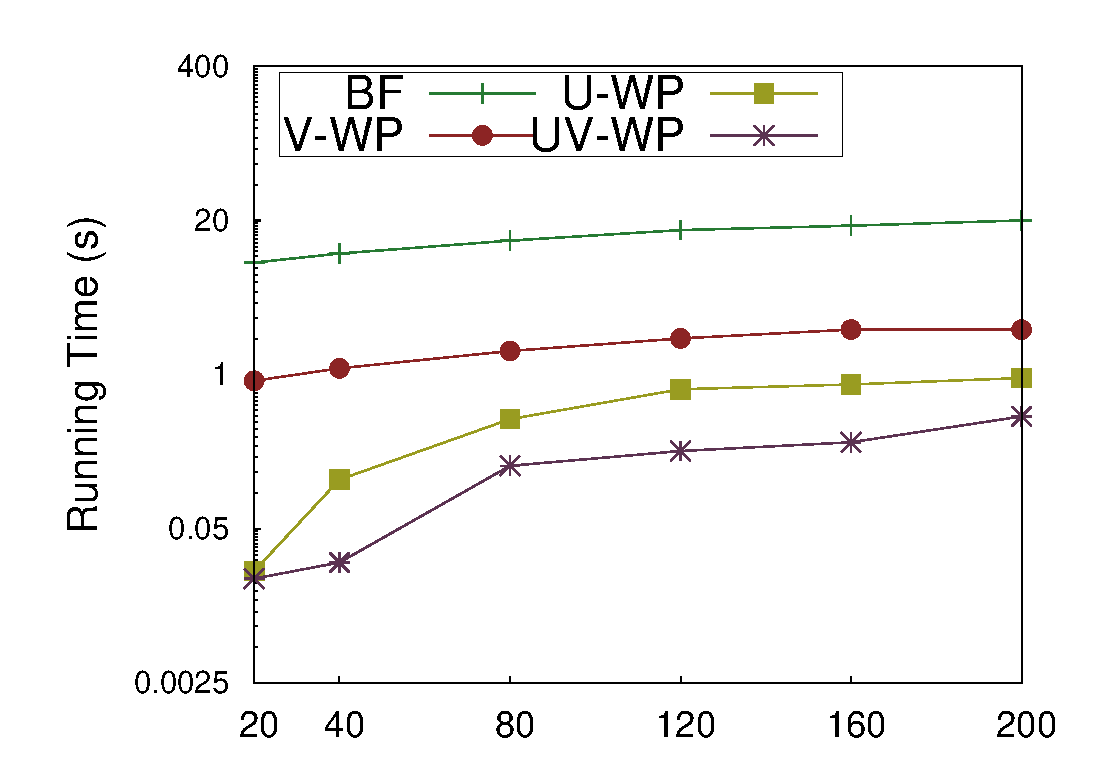
\includegraphics[width=\textwidth]{chapter4/exp/offline/varyp/nba_vary_p.eps}
        \caption{NBA}
    \end{subfigure}
    \begin{subfigure}[b]{0.45\textwidth}
        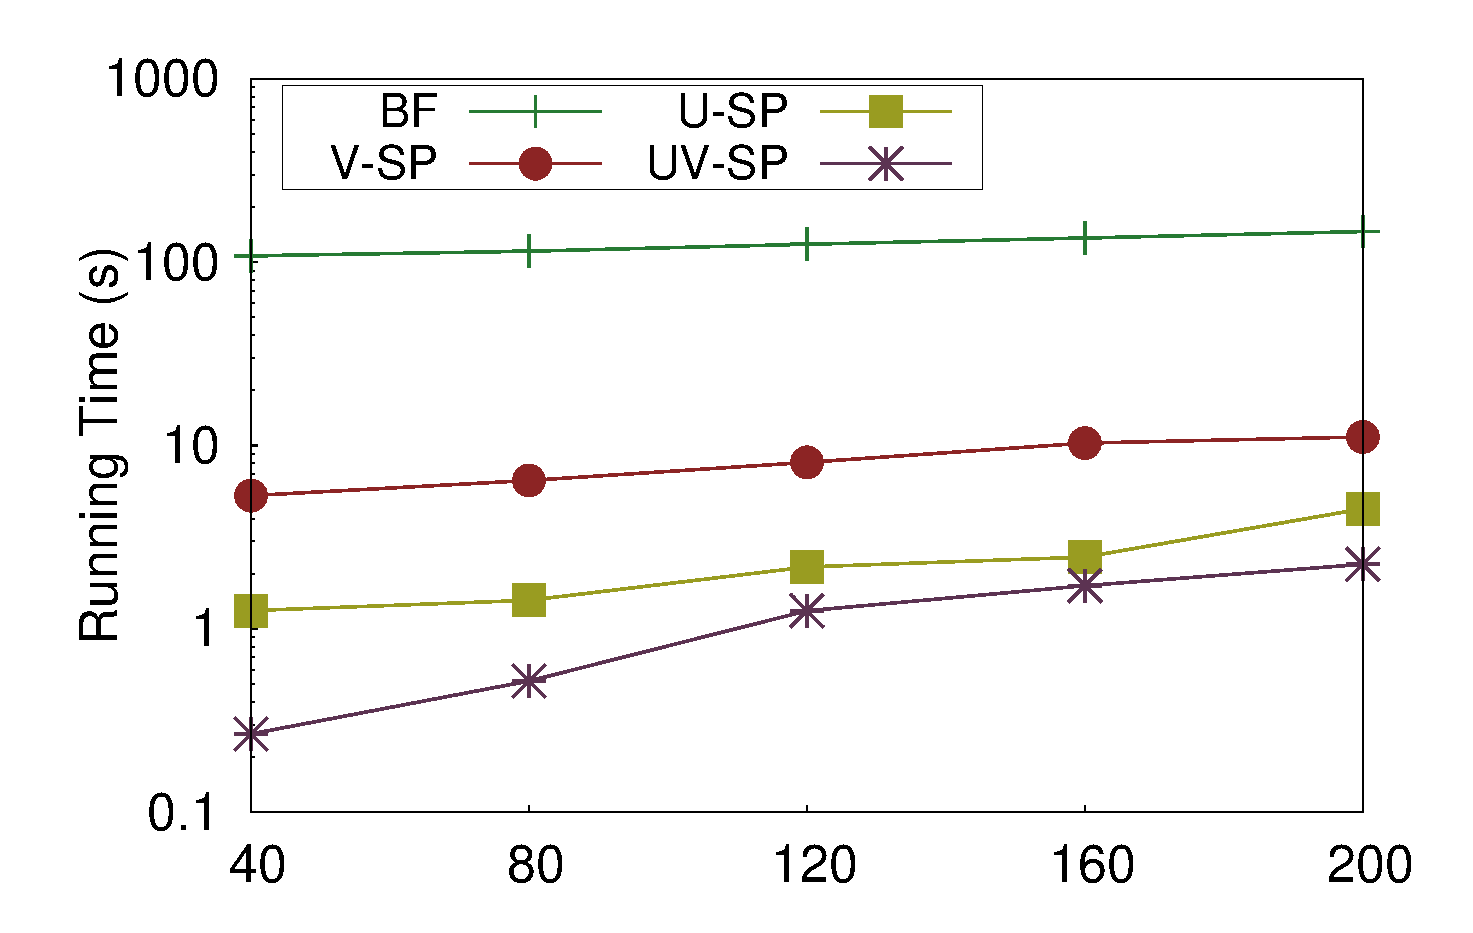
\includegraphics[width=\textwidth]{chapter4/exp/offline/varyp/power_vary_p.eps}
        \caption{POWER}
    \end{subfigure}
    \begin{subfigure}[b]{0.45\textwidth}
        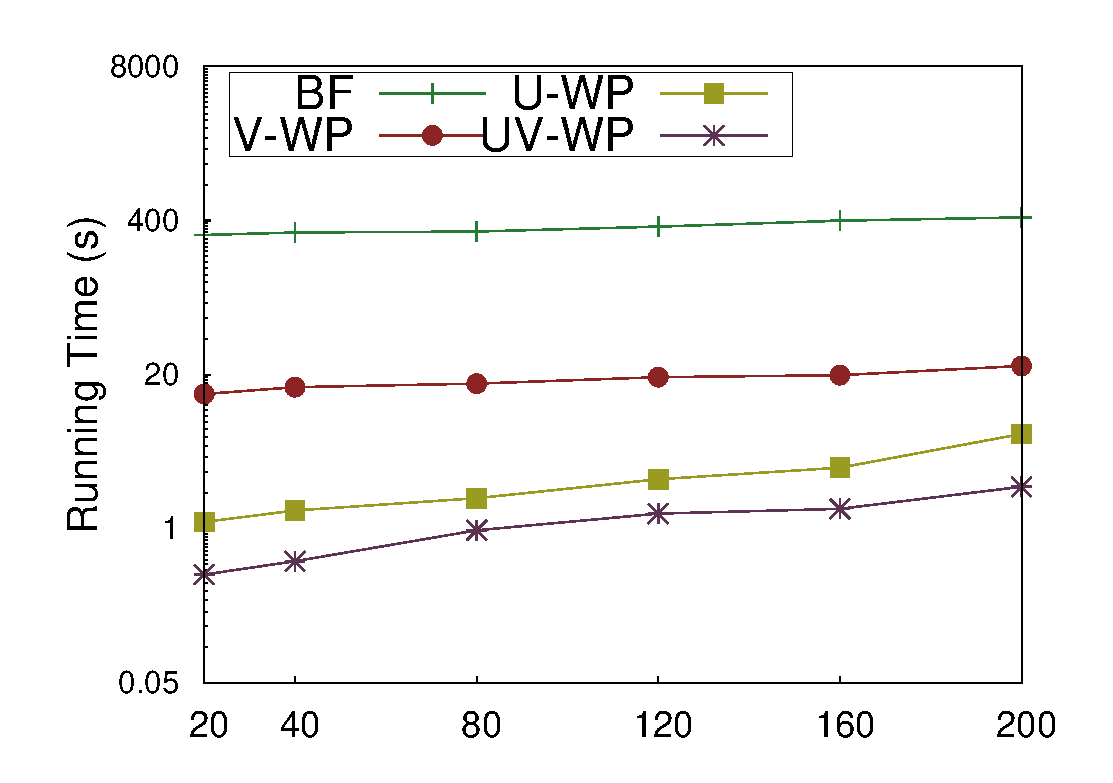
\includegraphics[width=\textwidth]{chapter4/exp/offline/varyp/stock_vary_p.eps}
        \caption{STOCK}
    \end{subfigure}
    \begin{subfigure}[b]{0.45\textwidth}
        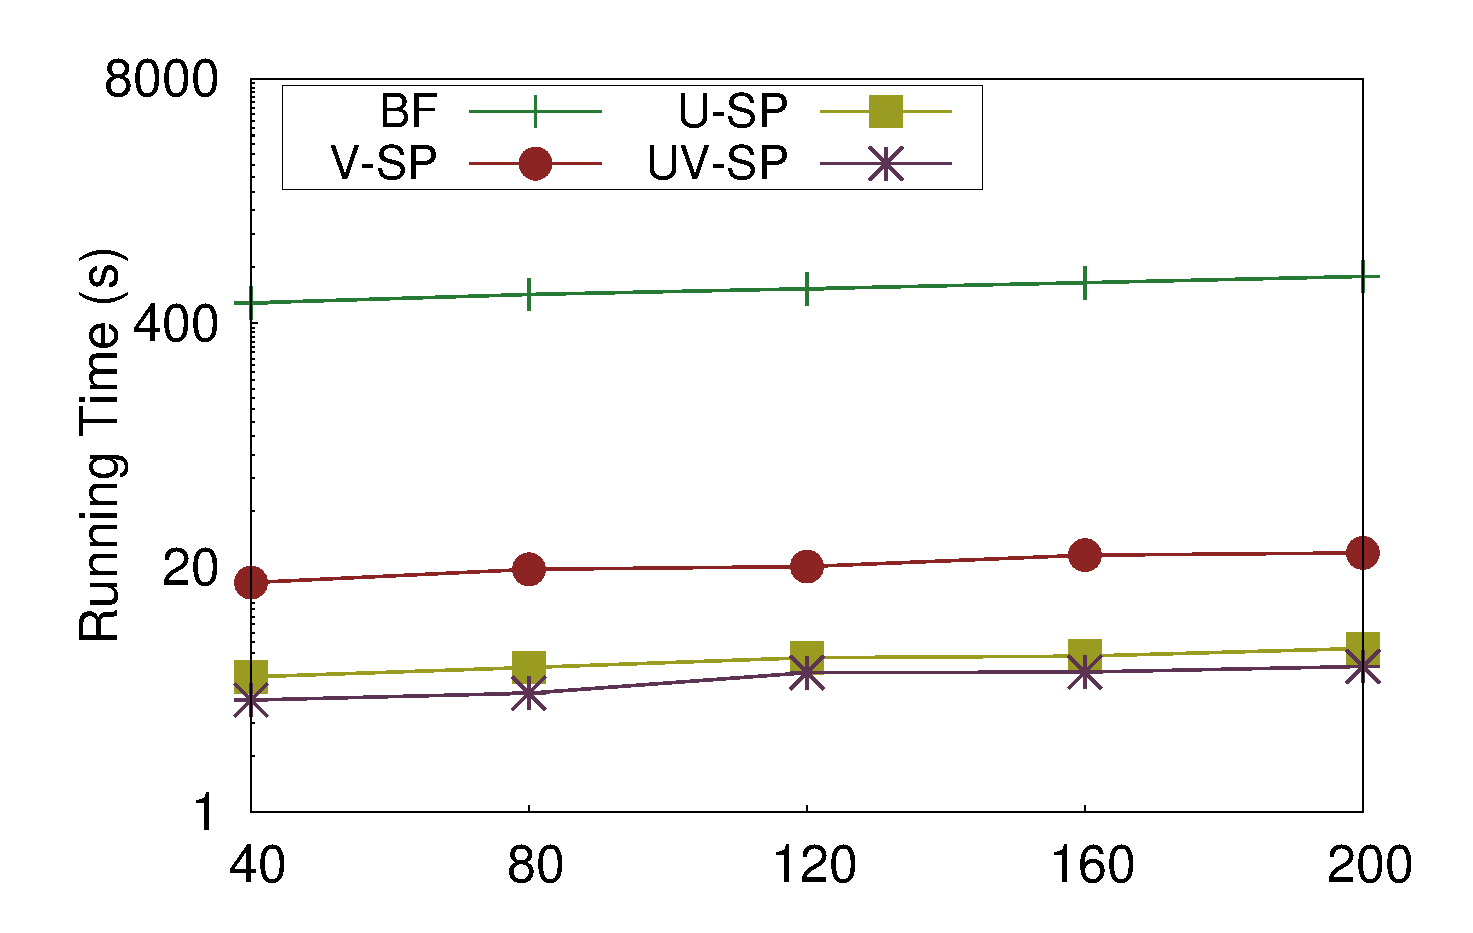
\includegraphics[width=\textwidth]{chapter4/exp/offline/varyp/pems_vary_p.eps}
        \caption{PEMS}
    \end{subfigure}
\caption{Candidate theme generation in the offline scenario with varying $p$.}
\label{exp:offline_performance_vary_p}
\end{figure*}

\subsubsection{Candidate theme generation with varying $h$}
We then study the performance of four algorithms wrt. the number of events and report the results 
in Fig.~\ref{exp:offline_performance_vary_n}. As presented in the figures, when $h$ increases, 
the running time for all the four algorithms also increases. This is because more event windows need to be evaluated. 
Again, pruning-based methods are much efficient than the baseline method. When both pruning methods are adapted, our method obtains hundreds of times faster than the baseline method.


\subsubsection{Sketch discovery with varying $k$}
After candidate themes are generated, we greedily find the $k$-sketch for each subject. 
Here, we study the effect of $k$ on the performance of the greedy algorithm. The results on four datasets are presented in Table~\ref{exp:offline_greedy}. The table indicates that for all four datasets, as $k$ increases, the running time of the greedy algorithm proportionally increases. This is because the complexity of the greedy algorithm is $O(k\Sigma_s|\mathbb{N}_s|)$. Since PEMS is the largest dataset with highest $\Sigma_s|\mathbb{N}_s|$, greedy algorithm performs worst on PEMS. As we observe that, even greedy algorithm takes upto 400 seconds on PEMS, the performance of the exact solution with quadratic complexity is not acceptable. This confirms the necessity of adapting the approximation algorithm.
%
%We can see that greedy algorithm perform worst on PEMS. When $k$ increases, its performance degrades dramatically. 
%This is because PEMS is the largest dataset, while the complexity of the greedy algorithm is $O(k\Sigma_s|\mathbb{N}_s|)$. As PEMS has a highest ratio of $\Sigma_s|\mathbb{N}_s|$

%thus the performance of greedy algorithm is more sensitive to $k$.


%We can see that PEMS is the largest dataset and thus is most sensitive to $k$. When $k$ increases, its performance degrades dramatically because the complexity of the greedy algorithm is $O(k\Sigma_s|\mathbb{N}_s|)$ and its ratio $\Sigma_s|\mathbb{N}_s|$ is higher than the other three datasets. This also explains why the performance in NBA dataset remains quite stable when $k$ increases.

\begin{figure*}[t]
\centering
    \begin{subfigure}[b]{0.45\textwidth}
        \includegraphics[width=\textwidth]{chapter4/exp/offline/varyh/nba_varyh.eps}
        \caption{NBA}
    \end{subfigure}
    \begin{subfigure}[b]{0.45\textwidth}
        \includegraphics[width=\textwidth]{chapter4/exp/offline/varyh/power_varyh.eps}
        \caption{POWER}
    \end{subfigure}
    \begin{subfigure}[b]{0.45\textwidth}
        \includegraphics[width=\textwidth]{chapter4/exp/offline/varyh/stock_varyh.eps}
        \caption{STOCK}
    \end{subfigure}
    \begin{subfigure}[b]{0.45\textwidth}
        \includegraphics[width=\textwidth]{chapter4/exp/offline/varyh/pems_varyh.eps}
        \caption{PEMS}
    \end{subfigure}
\caption{Candidate theme generation in the offline scenario with varying $h$.}
\label{exp:offline_performance_vary_n}
\end{figure*}

%\begin{figure}[h]
%\centering
%        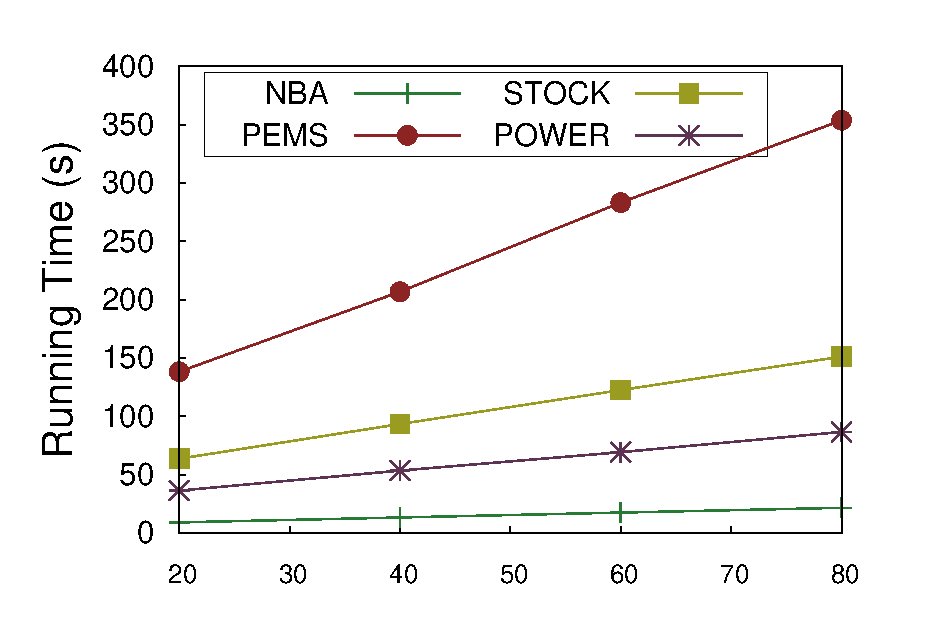
\includegraphics[width=0.25\textwidth]{offline/greedy/offline_varyk.eps}
%\caption{Greedy algorithm performance in offline sketch discovery with varying $k$}
%\label{exp:offline_greedy}
%\end{figure}

{\renewcommand{\arraystretch}{1.2} 
\begin{table}
\small
\centering
\caption{Sketch discovery with varying $k$ in (ms)}\label{exp:offline_greedy}
\begin{tabular}{|c|c|c|c|c|c|}
\hline 
\textbf{k} & \textbf{20} & \textbf{40} & \textbf{60} & \textbf{80}& \textbf{100} \\ 
\hline 
NBA & 9,097 & 13,345	& 17,500	& 21,597 & 	30,769 \\ 
\hline 
POWER & 36,297 & 53,513 & 69,300 &	86,603 &	122,856
\\ 
\hline 
STOCK & 63,679	& 93,415 &	122,500 &	151,179 &	215,386\\ 
\hline 
PEMS & 138,224	& 206,820 &	283,190 &	353,766	& 491,000 \\ 
\hline 
\end{tabular} 
\end{table}
}



\subsection{Online Sketch Maintenance}
\label{subsec:exp-online}
In the online scenario, we evaluate the following four algorithms to make performance comparisons:

\noindent\textbf{Sketch Computing (SC)}: SC examines all event windows generated from a fresh event.  Whenever there is an update in any subject's sketch, Algorithm~\ref{algo:greedy} will be invoked. To improve efficiency, the updates are processed in a batch manner, i.e., multiple updates
on the same subject will be batched and processed by calling Algorithm~\ref{algo:greedy} once.

\noindent\textbf{Sketch with Early Termination (SET)}: SET adopts ``Online Window Bound'' in Theorem~\ref{thm:online_bound} for early termination.

\noindent\textbf{Approx. Sketch (AS)}: AS is similar to \emph{SC} except that it only computes the approximate sketches. 

\noindent\textbf{Approx. Sketch with Early Termination (ASET)}: ASET computes the approximate sketches with early termination, as shown in Algorithm~\ref{algo:online_overview}.

In the online setting, we are more interested in evaluating the throughput of algorithms. We report the performance wrt. $p$, $k$ and $h$.


\subsubsection{Query throughput with varying $p$}
We increase $p$ from 10 to 200 and the throughput results are 
shown in Fig.~\ref{exp:online_mining_vary_P}.
Figs.~\ref{exp:online_mining_vary_P} (a)-(d) show that all four datasets
demonstrate similar patterns. As $p$ increases, 
the throughput of the four algorithms drops.
This is because as $p$ increases, the time to maintain the $p$ best candidate themes
as well as to update the sketch increases. However, algorithms adapting 
\emph{online window bound} have higher throughput than their counterparts. 
This is because with early termination, fewer candidate themes are generated. 
We can also see that $SC$ and $ASC$ run very slow in the online setting. 
This is because they need to invoke Algorithm~\ref{algo:greedy} upon every update.
This confirms the necessity of our approximation method as $ASET$ achieves up to 500x boosts as compared to $SC$.

\begin{figure*}[t]
\centering
    \begin{subfigure}[b]{0.45\textwidth}
        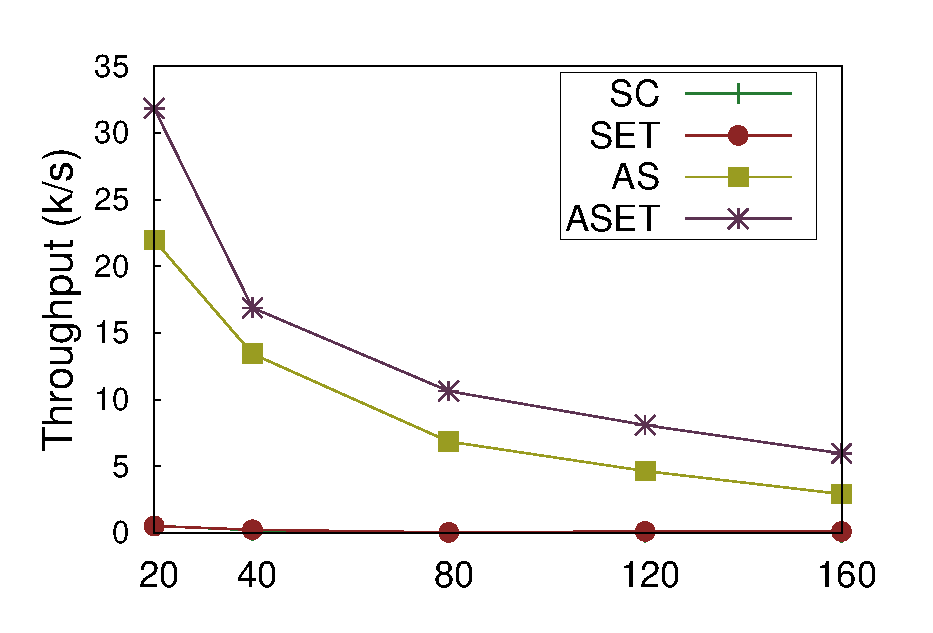
\includegraphics[width=\textwidth]{chapter4/exp/online/varyp/nba_varyp.eps}
        \caption{NBA}
    \end{subfigure}
    \begin{subfigure}[b]{0.45\textwidth}
        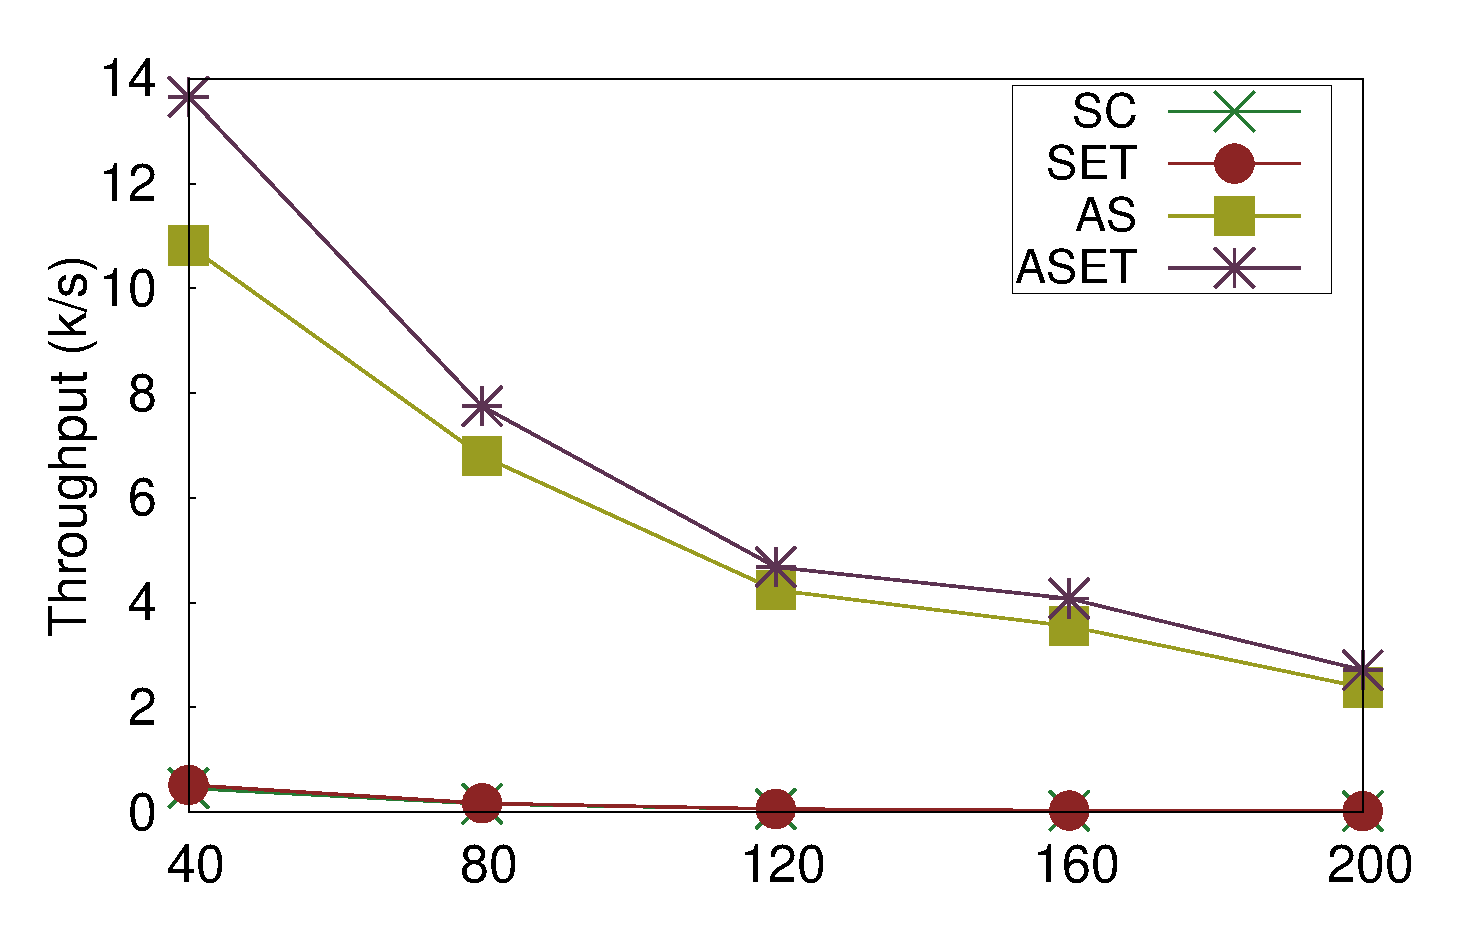
\includegraphics[width=\textwidth]{chapter4/exp/online/varyp/power_varyp.eps}
        \caption{POWER}
    \end{subfigure}
    \begin{subfigure}[b]{0.45\textwidth}
        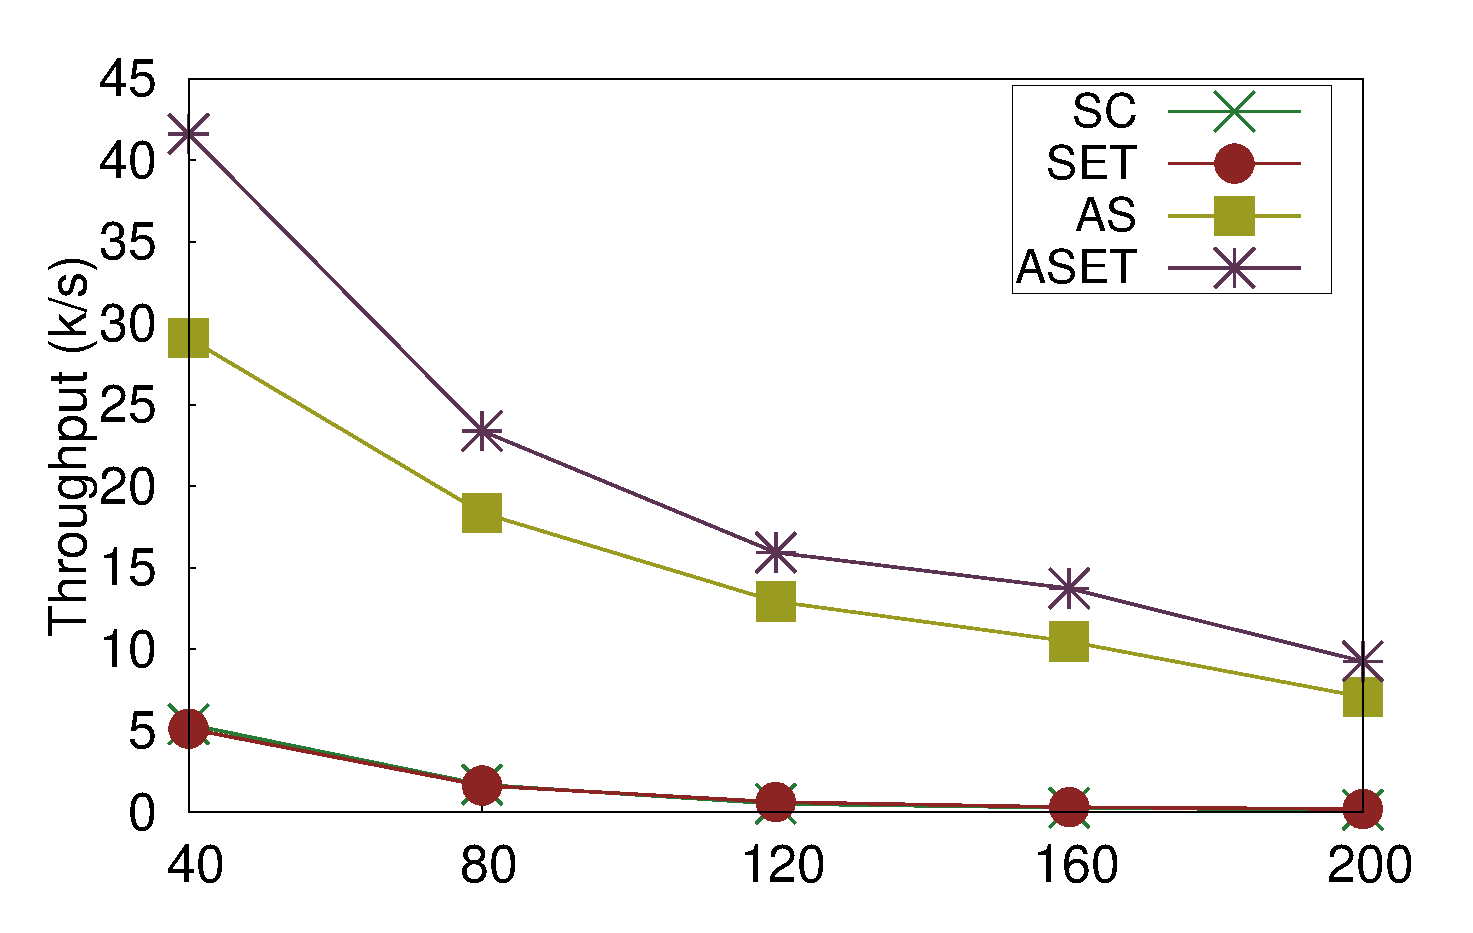
\includegraphics[width=\textwidth]{chapter4/exp/online/varyp/stock_varyp.eps}
        \caption{STOCK}
    \end{subfigure}
    \begin{subfigure}[b]{0.45\textwidth}
        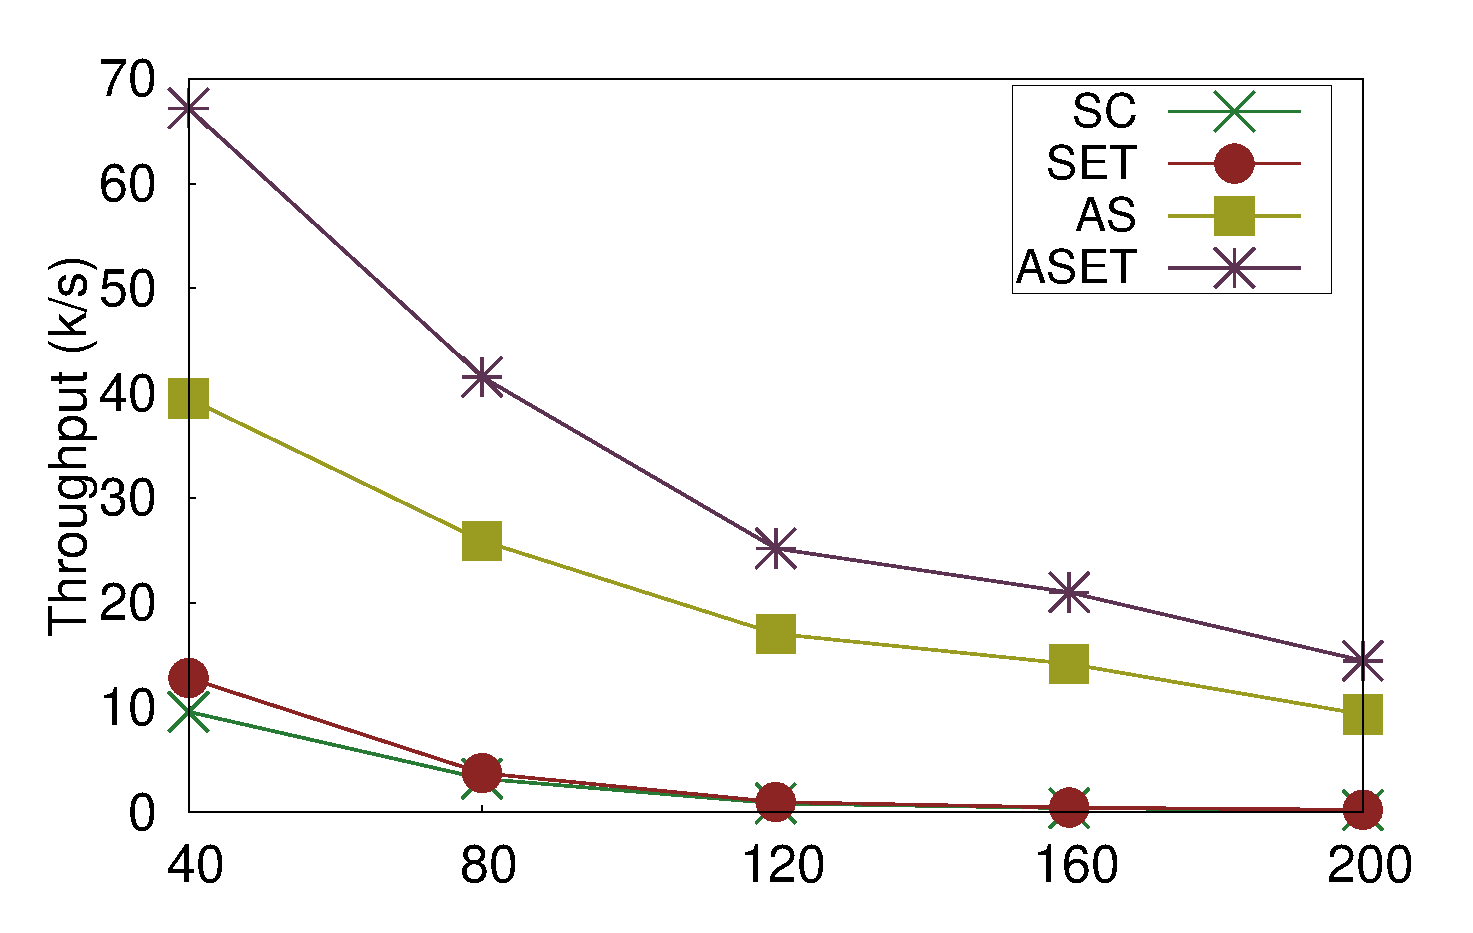
\includegraphics[width=\textwidth]{chapter4/exp/online/varyp/pems_varyp.eps}
        \caption{PEMS}
    \end{subfigure}
\caption{Throughput in online scenario with varying $p$.}
\label{exp:online_mining_vary_P}
\end{figure*}

\subsubsection{Query throughput with varying $k$} 
We then evaluate how the throughput varies wrt. $k$. 
The results are presented in Fig.~\ref{exp:online_mining_vary_k}.
The figures tell similar patterns as
Figs.~\ref{exp:online_mining_vary_P}.
First, as $k$ increases, the throughput of all the four algorithms decreases.
This is because as $k$ becomes large, more operations are needed for maintaining the sketch.
Second, the throughput of $SC$ and $SET$ are order of magnitudes smaller than $AS$ and $ASET$.
This is because of the repetitive calling of Algorithm~\ref{algo:greedy} for each arrival event,
which heavily depends on $k$. We observe that in some datasets (e.g., Fig.~\ref{exp:online_mining_vary_k} (a)) there is a hundreds time boost for $ASET$ as compared to $SC$.

\begin{figure}[t]
\centering
    \begin{subfigure}[b]{0.45\textwidth}
        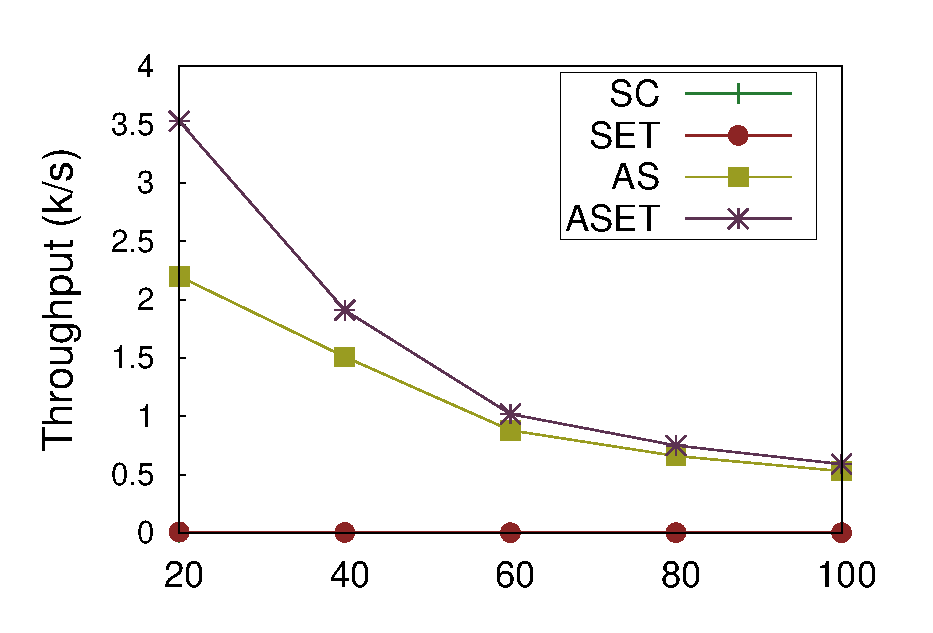
\includegraphics[width=\textwidth]{chapter4/exp/online/varyk/nba_varyk.eps}
        \caption{NBA}
    \end{subfigure}
    \begin{subfigure}[b]{0.45\textwidth}
        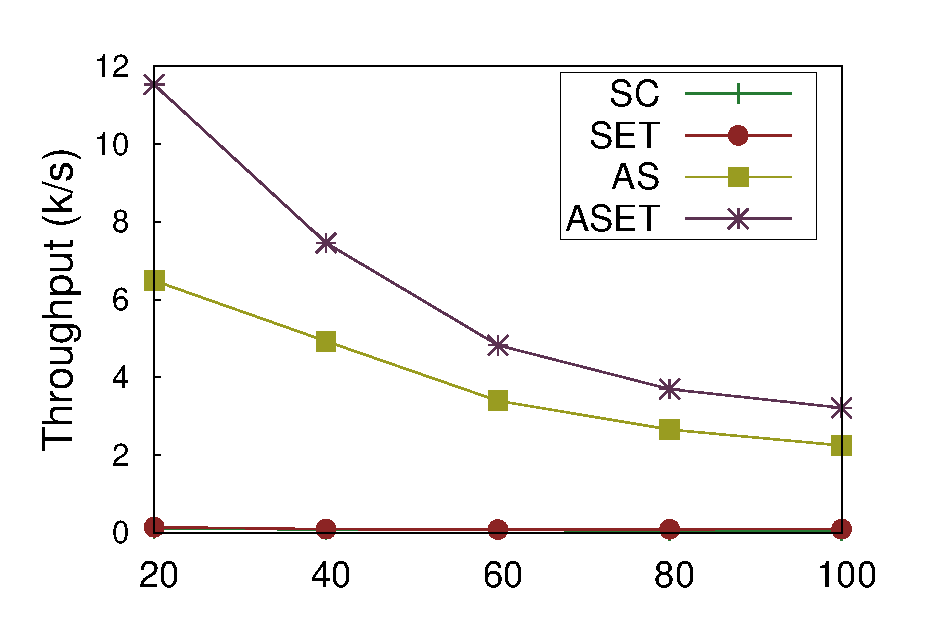
\includegraphics[width=\textwidth]{chapter4/exp/online/varyk/power_varyk.eps}
        \caption{POWER}
    \end{subfigure}
    \begin{subfigure}[b]{0.45\textwidth}
        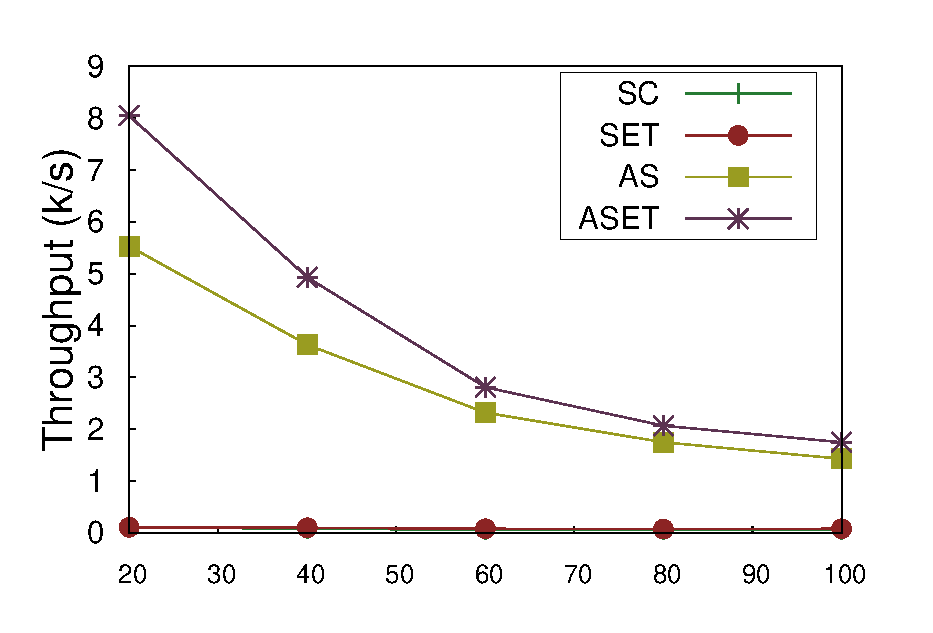
\includegraphics[width=\textwidth]{chapter4/exp/online/varyk/stock_varyk.eps}
        \caption{STOCK}
    \end{subfigure}
    \begin{subfigure}[b]{0.45\textwidth}
        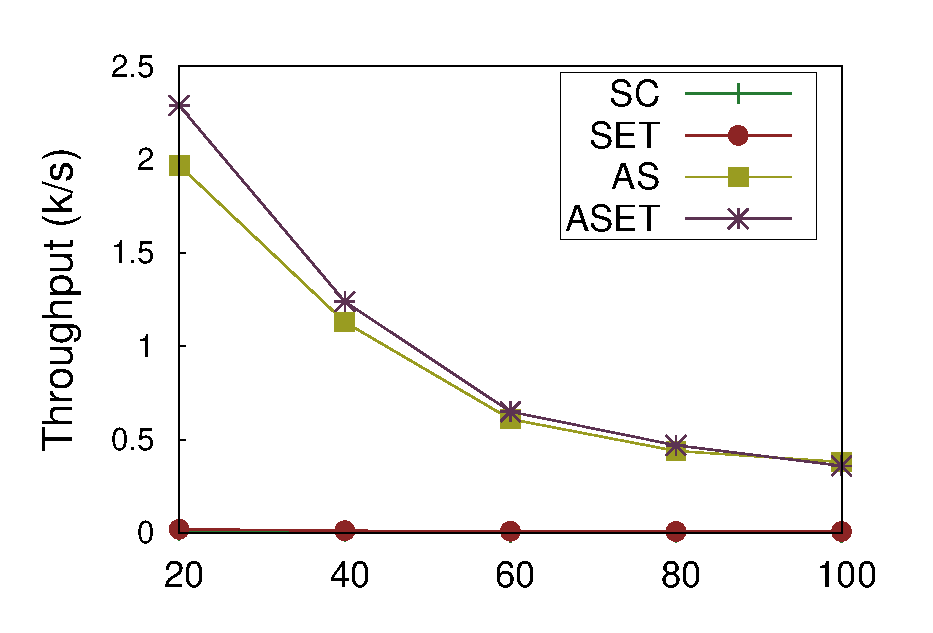
\includegraphics[width=\textwidth]{chapter4/exp/online/varyk/pems_varyk.eps}
        \caption{PEMS}
    \end{subfigure}
\caption{Throughput in online scenario with varying $k$.}
\label{exp:online_mining_vary_k}
\end{figure}

\subsubsection{Query throughput with varying $h$}
Finally we study the effect of $h$ in affecting algorithm throughput online.
We change $h$ from 20 to 100, and the results are in Fig.~\ref{exp:online_mining_vary_h}.
As shown in the figures, when $h$ increases, 
the throughput of the four algorithms steady drops.
This is because as $h$ increases, $|\mathbb{H}_s|$ for each subject
increases. Therefore, in Algorithm~\ref{algo:online_overview}, more time is needed 
to process each event window. We notice that \emph{ASET} has a flatter slope than \emph{AS}; this
dues to the benefit from the prunings of \emph{online window bound}.
\begin{figure}[t]
\centering
    \begin{subfigure}[b]{0.45\textwidth}
        \includegraphics[width=\textwidth]{chapter4/exp/online/varyh/nba_varyh.eps}
        \caption{NBA}
    \end{subfigure}
    \begin{subfigure}[b]{0.45\textwidth}
        \includegraphics[width=\textwidth]{chapter4/exp/online/varyh/power_varyh.eps}
        \caption{POWER}
    \end{subfigure}
    \begin{subfigure}[b]{0.45\textwidth}
        \includegraphics[width=\textwidth]{chapter4/exp/online/varyh/stock_varyh.eps}
        \caption{STOCK}
    \end{subfigure}
    \begin{subfigure}[b]{0.45\textwidth}
        \includegraphics[width=\textwidth]{chapter4/exp/online/varyh/pems_varyh.eps}
        \caption{PEMS}
    \end{subfigure}
\caption{Throughput in online scenario with varying $h$.}
\label{exp:online_mining_vary_h}
\end{figure}


\subsection{Comparison with Other Techniques}
\label{subsec:exp-survey}
We also compare both the performance and effectiveness of our sketch discovery with prominent streak
technique~\cite{zhang2014discovering} (denoted by skyline method). Due to the mismatched goal of sketch and skyline, these experiments only serve as references.

To study the efficiency, we first modify the skyline technique in~\cite{zhang2014discovering} to consider ranks. In the offline scenario, the rank is computed using BF method, while in the online scenario, we directly keep the $WI$ and the rank can be easily maintained. We use the default parameters settings for both scenarios. Figs.~\ref{exp:sky_comp} (a)(b) show the running time comparisons under all four datasets. We can see that, when trying to adapt for rank-awareness, naively computing the rank on skyline method incurs high overheads. For instance, as presented in Fig.~\ref{exp:sky_comp} (a), in the offline scenario, the running time of skyline method is order of magnitude slower than sketch method. This supports the use of pruning techniques in computing the ranks. Similarly, as shown in Fig.~\ref{exp:sky_comp} (b), in the online scenario, our sketch method still has a much better throughput. Although skyline method is free from passive update, as it is computationally expensive to maintain online skyline points, we still observe an upto 5 times boosts of sketch method.


To study the effectiveness, we conduct a user study over Amazon Mechanical Turk~\footnote{https://requester.mturk.com} to evaluate the attractiveness of the $k$-sketch. For our method, we set $p=200$ to allow more candidate themes and set $\alpha=0.5$ to pay equal attention to strikingness and diversity. For the skyline method, due to the overwhelming skyline points generated for each subject, we propose three augmented methods to pick $k$ of them. In total, we have the following five algorithms to compare with:
\begin{enumerate}
\setlength\itemsep{-0.1cm}
\item{$SK$: selects the $k$-sketch for each player generated by offline sketch discovery method.}
\item{$SK_a$: selects the $k$-sketch for each player generated by online approximate sketch method;}
\item{$SY_s$: randomly selects $k$ streaks for each player from the bunch of skylines generated by~\cite{zhang2014discovering};}
\item{$SY_m$: selects $k$ streaks sorted by freshness of the events;}
\item{$SY_r$: selects $k$ rank-attached streaks sorted by
the scoring function proposed in this paper;}
\end{enumerate}

In our experimental setting, we use the NBA dataset and set $k=20$ to generate $20$ news themes for each player. Each news theme is in the following format:

\textit{[2003-04-14]: Michael-Jordan scored an average of 30.30 pts for 989 straight games,which is No. 1 in NBA history!!}

Thus, each algorithm results in $20$ news themes for each player. We design each job in AMT to contain $20$ questions. For each question, we randomly pick one unchosen news theme from each algorithm. So each question contains $5$ news and we require users to pick the most attractive one in each question. We received responses from 202 participants who have knowledge in NBA\footnote{In AMT, we are able to request respondents with certain qualifications, i.e. knowledgeable in NBA.}. Then, for each algorithm, we count the frequency of being selected as the most attractive and report the percentage results in the pie chart in Fig.~\ref{exp:survey}.  

The charts clearly shows that $SK$ is the most effective method as $45\%$
of its generated news are considered as the most attractive. Interestingly, we observe
that there are respondents who choose other comparing methods as their favorites. Besides human noise, 
we note that a portion of the news themes, which get votes and are generated by the comparing methods, 
overlap with news themes produced by our sketch based approach. In fact, $SK_a$ overlaps $52\%$ of event 
windows with $SK$. Thus it ranked as the second most attractive. Whereas $SY_s$ overlaps only $10\%$ event windows
with $SK$, it is ranked last. The chart also shows that the ranking based on freshness $SY_m$
can slightly improve the attractiveness compared with $SY_s$. However, when applied with our proposed ranking function(i.e., $SY_r$), the number of respondents preferring the ranked skyline results increases dramatically, nearly two times of the original number of respondents. This also implies the effectiveness of our scoring function.

%Meanwhile, its approximate variant $SK_a$ in the online scenario also achieved good performance and ranked as the second most attractive.
%Without any ranking, the skyline streak method~\cite{zhang2014discovering} gets the worst performance. We observe that there are still near 20\% responses pick skyline streaks as top-interesting. This is because the news themes generated by sketch and skyline have overlaps. For example, the news ``Michael Jordan has an average points of 30.30 for 989 games'' appears in the theme results of all five algorithms. In fact, we notice 24\% overlapped event windows between sketch and skyline methods. Under such circumstances, users may choose at random, which explains the 20\% responses for skyline streaks.
%The ranking based on freshness can slightly improve the attractiveness. However, when applied with our proposed ranking function, the number of users preferring the ranked skyline results increases dramatically, nearly two times of the original number of users. This also implies the effectiveness of our scoring function.

\begin{figure}[t]
\centering
    \begin{subfigure}[b]{0.45\textwidth}
        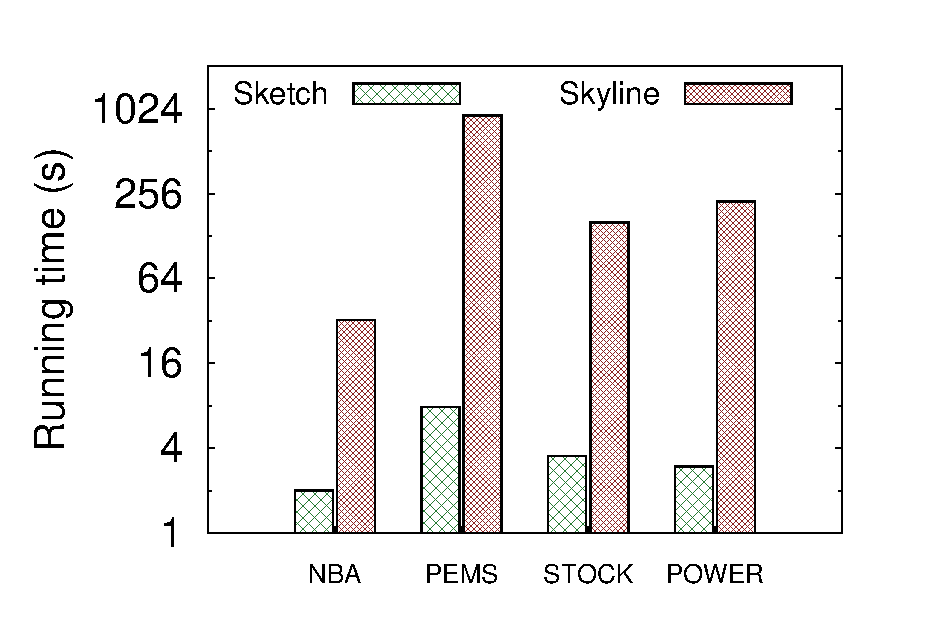
\includegraphics[width=\textwidth]{chapter4/exp/sky_comp/sky_comp_offline.eps}
        \caption{Offline Scenario}
    \end{subfigure}
    \begin{subfigure}[b]{0.45\textwidth}
        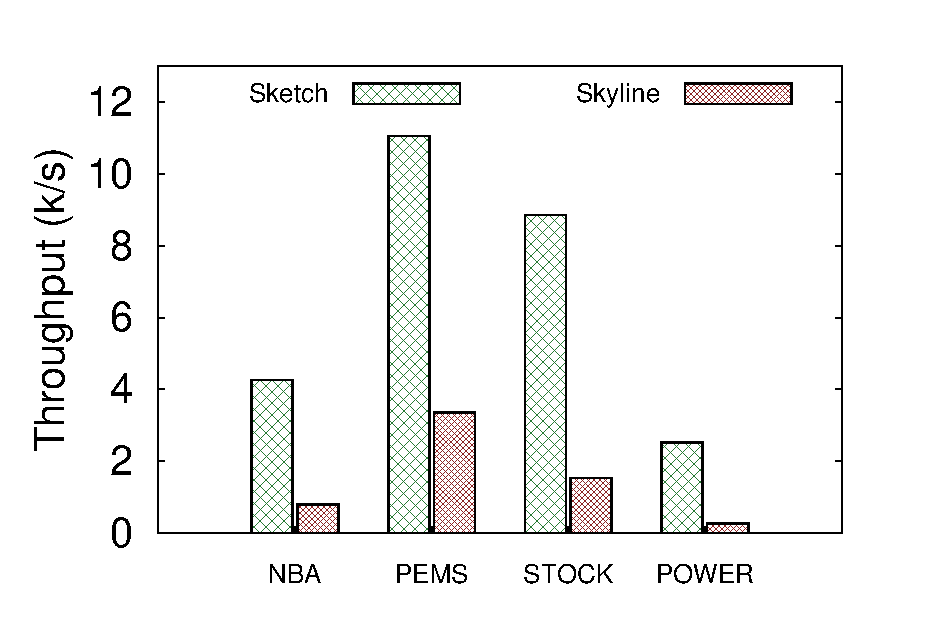
\includegraphics[width=\textwidth]{chapter4/exp/sky_comp/sky_comp_online.eps}
        \caption{Online Scenario}
    \end{subfigure}
\caption{Efficiency comparison with existing technique}
\label{exp:sky_comp}
\end{figure}

\begin{figure}[h]
\centering
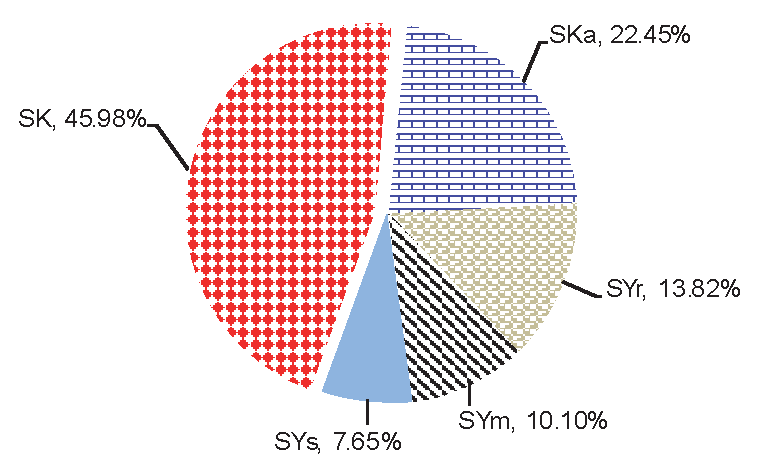
\includegraphics[width=0.4\textwidth]{chapter4/exp/survey/survey.eps}
\caption{Percentage of news considered as the most attractive.}
\label{exp:survey}
\end{figure}




